\documentclass[11pt]{article}
\usepackage[letterpaper, margin=0.6in, top=0.65in, bottom=0.45in]{geometry}
\usepackage{amsmath, amssymb}
\usepackage{xcolor}
\usepackage{tikz}
\usepackage{fancyhdr}

\pagestyle{fancy}
\fancyhf{}
\fancyhead[L]{\small\textbf{CSSE 490 --- Deep Reinforcement Learning}}
\fancyhead[R]{\small\textbf{Lecture 13: Backpropagation}}
\fancyfoot[C]{\thepage}
\renewcommand{\headrulewidth}{0.4pt}

\newcommand{\blk}[1]{\underline{\hspace{#1}}}
\setlength{\parindent}{0pt}
\setlength{\parskip}{2pt}
\setlength{\abovedisplayskip}{4pt}
\setlength{\belowdisplayskip}{4pt}
\setlength{\abovedisplayshortskip}{2pt}
\setlength{\belowdisplayshortskip}{2pt}

\begin{document}


\begin{center}
{\Large \textbf{Backpropagation Handout}}\\[2pt]
{\normalsize Step-by-Step Feedforward \& Backpropagation}
\end{center}


\vspace{-2pt}
\begin{center}
\fbox{\parbox{0.92\textwidth}{\small
\textbf{Your Tasks:}\;
\textbf{Forward:} compute all intermediate values $H$, $L$, $O$, $Y$, $\mathcal{L}$ (Steps 1--5). \quad
\textbf{Backward:} compute $\partial\mathcal{L}/\partial w^b_{21}$ and
$\partial\mathcal{L}/\partial w^a_{11}$.
}}
\end{center}


\vspace{-2pt}\hrule\vspace{4pt}

\textbf{Setup}\; {\small (from \texttt{BackProp.py})}

\vspace{1pt}
\begin{tabular}{@{}rl@{\qquad\qquad}rl@{}}
\textbf{Input:} & $x = (0.9,\; 0.5,\; 0.1)^T$ &
\textbf{Target:} & $y = (1,\; 0)^T$ \\[2pt]
$W_a$: & $4\!\times\!3$, no bias, all entries $= 0.1$ &
$W_b$: & $2\!\times\!4$, no bias, all entries $= 0.1$ \\
\end{tabular}


\begin{center}
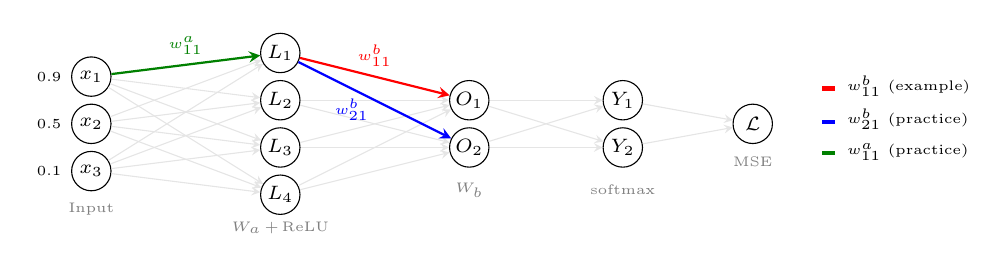
\begin{tikzpicture}[x=1.5cm, y=0.6cm,
  n/.style={circle, draw, minimum size=5mm, inner sep=0pt, font=\scriptsize},
  >=stealth]

% Input layer
\node[n] (x1) at (0,1) {$x_1$};
\node[n] (x2) at (0,0) {$x_2$};
\node[n] (x3) at (0,-1) {$x_3$};

% Hidden layer (H -> ReLU -> L combined)
\node[n] (l1) at (1.6, 1.5) {$L_1$};
\node[n] (l2) at (1.6, 0.5) {$L_2$};
\node[n] (l3) at (1.6,-0.5) {$L_3$};
\node[n] (l4) at (1.6,-1.5) {$L_4$};

% Output layer
\node[n] (o1) at (3.2, 0.5) {$O_1$};
\node[n] (o2) at (3.2,-0.5) {$O_2$};

% Y layer
\node[n] (y1) at (4.5, 0.5) {$Y_1$};
\node[n] (y2) at (4.5,-0.5) {$Y_2$};

% Loss
\node[n] (loss) at (5.6, 0) {$\mathcal{L}$};

% Gray connections: x -> l
\foreach \a in {1,2,3} { \foreach \b in {1,...,4} { \draw[gray!20, ->] (x\a)--(l\b); } }
% Gray connections: l -> o
\foreach \a in {1,...,4} { \foreach \b in {1,2} { \draw[gray!20, ->] (l\a)--(o\b); } }
% Gray connections: o -> y
\foreach \a in {1,2} { \foreach \b in {1,2} { \draw[gray!20, ->] (o\a)--(y\b); } }
% Gray connections: y -> loss
\foreach \a in {1,2} { \draw[gray!20, ->] (y\a)--(loss); }

% Highlighted weight edges
\draw[red, thick, ->] (l1)--(o1)
  node[midway, above, font=\tiny, text=red] {$w^b_{11}$};
\draw[blue, thick, ->] (l1)--(o2)
  node[pos=0.35, below, font=\tiny, text=blue] {$w^b_{21}$};
\draw[green!50!black, thick, ->] (x1)--(l1)
  node[midway, above, font=\tiny, text=green!50!black] {$w^a_{11}$};

% Layer labels
\node[font=\tiny, gray] at (0, -1.8) {Input};
\node[font=\tiny, gray] at (1.6, -2.2) {$W_a$\,+\,ReLU};
\node[font=\tiny, gray] at (3.2, -1.4) {$W_b$};
\node[font=\tiny, gray] at (4.5, -1.4) {softmax};
\node[font=\tiny, gray] at (5.6, -0.8) {MSE};

% Input values
\node[left, font=\tiny] at (x1.west) {0.9};
\node[left, font=\tiny] at (x2.west) {0.5};
\node[left, font=\tiny] at (x3.west) {0.1};

% Legend
\node[right, font=\tiny, anchor=west] at (6.1, 0.8)
  {\textcolor{red}{\rule{5pt}{1.5pt}}\; $w^b_{11}$ (example)};
\node[right, font=\tiny, anchor=west] at (6.1, 0.1)
  {\textcolor{blue}{\rule{5pt}{1.5pt}}\; $w^b_{21}$ (practice)};
\node[right, font=\tiny, anchor=west] at (6.1,-0.6)
  {\textcolor{green!50!black}{\rule{5pt}{1.5pt}}\; $w^a_{11}$ (practice)};

\end{tikzpicture}
\end{center}


\vspace{-6pt}\hrule\vspace{4pt}

{\large \textbf{Forward Pass}}
\vspace{2pt}


\textbf{Step 1:} $H = W_a \cdot x$ \quad {\small (hidden pre-activation)}

\[
H = \underbrace{\begin{pmatrix} 0.1 & 0.1 & 0.1 \\ 0.1 & 0.1 & 0.1 \\
      0.1 & 0.1 & 0.1 \\ 0.1 & 0.1 & 0.1 \end{pmatrix}}_{W_a}
\!\cdot\!
\underbrace{\begin{pmatrix} 0.9 \\ 0.5 \\ 0.1 \end{pmatrix}}_{x}
\!=\!\begin{pmatrix} \blk{3.2cm} \\ \blk{3.2cm} \\                \blk{3.2cm} \\ \blk{3.2cm} \end{pmatrix}\!=\!\begin{pmatrix} \blk{1.2cm} \\ \blk{1.2cm} \\ \blk{1.2cm} \\ \blk{1.2cm} \end{pmatrix}
\]


\textbf{Step 2:} $L = \text{ReLU}(H)$ \quad
{\small $\text{ReLU}(z)=\max(0,z)$}

\[
L = \text{ReLU}\!\!\begin{pmatrix} \blk{1.2cm} \\ \blk{1.2cm} \\ \blk{1.2cm} \\ \blk{1.2cm} \end{pmatrix}
= \begin{pmatrix} \blk{1.2cm} \\ \blk{1.2cm} \\ \blk{1.2cm} \\ \blk{1.2cm} \end{pmatrix}
\]


\textbf{Step 3:} $O = W_b \cdot L$ \quad {\small (output pre-activation)}

\[
O = \underbrace{\begin{pmatrix} 0.1 & 0.1 & 0.1 & 0.1 \\
      0.1 & 0.1 & 0.1 & 0.1 \end{pmatrix}}_{W_b}
\!\cdot\!
\underbrace{\begin{pmatrix} 0.15 \\ 0.15 \\ 0.15 \\ 0.15 \end{pmatrix}}_{L}
\!=\! \begin{pmatrix} \blk{3.8cm} \\ \blk{3.8cm} \end{pmatrix} \!=\! \begin{pmatrix} \blk{1.2cm} \\ \blk{1.2cm} \end{pmatrix}
\]


\textbf{Step 4:} $Y = \text{softmax}(O)$ \quad
{\small $\displaystyle Y_i = \frac{e^{O_i}}{\sum_j e^{O_j}}$}

\[
Y_1 = \frac{e^{\blk{0.7cm}}}{e^{\blk{0.7cm}}+e^{\blk{0.7cm}}} = \blk{1.2cm}
\qquad
Y_2 = \blk{1.2cm}
\qquad\Rightarrow\quad
Y = \begin{pmatrix} \blk{1cm} \\ \blk{1cm} \end{pmatrix}
\]


\textbf{Step 5: MSE Loss}\quad
$\displaystyle\mathcal{L}=\tfrac{1}{N}\!\sum_{i=1}^{N}(y_i - Y_i)^2$\,,\ $N\!=\!2$

\[
\mathcal{L} = \tfrac{1}{2}\!\left[(\blk{0.6cm} - \blk{0.6cm})^2
+ (\blk{0.6cm} - \blk{0.6cm})^2\right]
= \blk{2.5cm} = \blk{1.2cm}
\]


\newpage
{\large \textbf{Backward Pass --- Per-Parameter Gradient Paths}}
\quad{\small We trace the \textbf{gradient path} backward from $\mathcal{L}$ to each
parameter, multiplying local derivatives along the way (chain rule).
At branches, we \textbf{sum} contributions from all paths.}
\vspace{2pt}



\vspace{-6pt}
{\small\textbf{Derivative formulas:}\;
MSE: $\frac{\partial\mathcal{L}}{\partial Y_i}\!=\!\frac{2}{N}(Y_i\!-\!y_i)$\;\;
Softmax: $\frac{\partial Y_i}{\partial O_j}\!=\!Y_i(\delta_{ij}\!-\!Y_j)$\;\;
Linear: $\frac{\partial O_i}{\partial w^b_{ij}}\!=\!L_j$,\;
$\frac{\partial O_i}{\partial L_j}\!=\!w^b_{ij}$,\;
$\frac{\partial H_i}{\partial w^a_{ij}}\!=\!x_j$\;\;
ReLU: $\frac{\partial L_i}{\partial H_i}\!=\!\mathbf{1}_{H_i>0}$}

\hrule\vspace{3pt}


\textbf{Example:} $\dfrac{\partial\mathcal{L}}{\partial w^b_{11}}$
\quad {\small\textcolor{red}{(red path: $w^b_{11}$ connects $L_1$ to $O_1$)}}
\vspace{-4pt}


\begin{center}\vspace{-2pt}
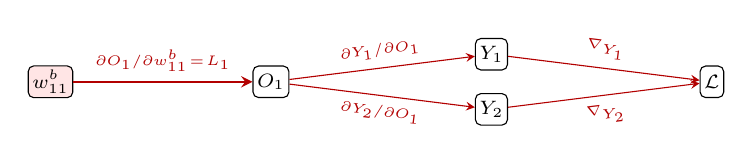
\begin{tikzpicture}[x=1.4cm, y=0.5cm,
  nd/.style={draw, rounded corners=2pt, minimum height=4mm,
             inner sep=1.5pt, font=\scriptsize},
  >=stealth]
\node[nd, fill=red!10] (w) at (0,0) {$w^b_{11}$};
\node[nd] (O) at (2,0) {$O_1$};
\node[nd] (Y1) at (4,0.7) {$Y_1$};
\node[nd] (Y2) at (4,-0.7) {$Y_2$};
\node[nd] (L) at (6,0) {$\mathcal{L}$};
\draw[->, red!70!black, thick] (w)--node[above,font=\tiny]{$\partial O_1/\partial w^b_{11}\!=\!L_1$}(O);
\draw[->, red!70!black] (O)--node[above,sloped,font=\tiny]{$\partial Y_1/\partial O_1$}(Y1);
\draw[->, red!70!black] (O)--node[below,sloped,font=\tiny]{$\partial Y_2/\partial O_1$}(Y2);
\draw[->, red!70!black] (Y1)--node[above,sloped,font=\tiny]{$\nabla_{Y_1}$}(L);
\draw[->, red!70!black] (Y2)--node[below,sloped,font=\tiny]{$\nabla_{Y_2}$}(L);
%\node[gray, font=\tiny] at (3,-1.1) {$\longleftarrow$ gradient flow};
\end{tikzpicture}\vspace{-4pt}
\end{center}


\vspace{-8pt}
{\small Derivatives along path:\;
$\frac{\partial\mathcal{L}}{\partial Y_k} = (Y_k\!-\!y_k)$,\quad
$\frac{\partial Y_k}{\partial O_1} = Y_k(\delta_{k1}\!-\!Y_1)$,\quad
$\frac{\partial O_1}{\partial w^b_{11}} = L_1$}
\vspace{-2pt}

\textbf{Values} {\small (used by all paths below):}\quad
{\small
$\nabla_{Y_1} = Y_1\!-\!y_1 = \blk{1cm}$,\;
$\nabla_{Y_2} = Y_2\!-\!y_2 = \blk{1cm}$}

\vspace{-4pt}
\begin{center}
{\small

$\frac{\partial Y_1}{\partial O_1}\!=\!\blk{1cm}$,\;
$\frac{\partial Y_2}{\partial O_1}\!=\!\blk{1cm}$,\;
$\frac{\partial Y_1}{\partial O_2}\!=\!\blk{1cm}$,\;
$\frac{\partial Y_2}{\partial O_2}\!=\!\blk{1cm}$
}
\end{center}
\begin{align*}
\frac{\partial\mathcal{L}}{\partial w^b_{11}}
&= \underbrace{\left[\blk{8cm}\right]}_{\nabla_{O_1}}
   \;\cdot\;\;
   \underbrace{\blk{3cm}}_{=\, L_1} \\[2pt]
&= \bigl[\blk{5cm}\bigr] \cdot \blk{1cm} \\
&= (\blk{1cm})(\blk{1cm}) = \blk{2cm}
\end{align*}


\vspace{-4pt}\hrule\vspace{2pt}
\textbf{Practice:} $\dfrac{\partial\mathcal{L}}{\partial w^b_{21}}$
\quad {\small\textcolor{blue}{(blue path: $w^b_{21}$ connects $L_1$ to $O_2$)}}
\vspace{-4pt}


\begin{center}\vspace{-2pt}
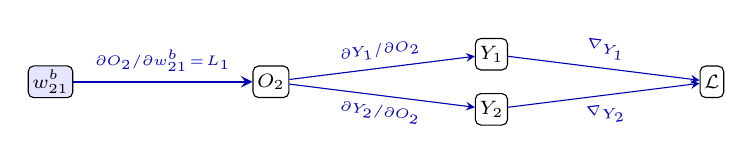
\begin{tikzpicture}[x=1.4cm, y=0.5cm,
  nd/.style={draw, rounded corners=2pt, minimum height=4mm,
             inner sep=1.5pt, font=\scriptsize},
  >=stealth]
\node[nd, fill=blue!10] (w) at (0,0) {$w^b_{21}$};
\node[nd] (O) at (2,0) {$O_2$};
\node[nd] (Y1) at (4,0.7) {$Y_1$};
\node[nd] (Y2) at (4,-0.7) {$Y_2$};
\node[nd] (L) at (6,0) {$\mathcal{L}$};
\draw[->, blue!70!black, thick] (w)--node[above,font=\tiny]{$\partial O_2/\partial w^b_{21}\!=\!L_1$}(O);
\draw[->, blue!70!black] (O)--node[above,sloped,font=\tiny]{$\partial Y_1/\partial O_2$}(Y1);
\draw[->, blue!70!black] (O)--node[below,sloped,font=\tiny]{$\partial Y_2/\partial O_2$}(Y2);
\draw[->, blue!70!black] (Y1)--node[above,sloped,font=\tiny]{$\nabla_{Y_1}$}(L);
\draw[->, blue!70!black] (Y2)--node[below,sloped,font=\tiny]{$\nabla_{Y_2}$}(L);
%\node[gray, font=\tiny] at (3,-1.1) {$\longleftarrow$ gradient flow};
\end{tikzpicture}\vspace{-4pt}
\end{center}


\vspace{-8pt}
{\small Derivatives along path:\;
$\frac{\partial\mathcal{L}}{\partial Y_k} = (Y_k\!-\!y_k)$,\quad
$\frac{\partial Y_k}{\partial O_2} = Y_k(\delta_{k2}\!-\!Y_2)$,\quad
$\frac{\partial O_2}{\partial w^b_{21}} = L_1$}
\vspace{-2pt}
\begin{align*}
\frac{\partial\mathcal{L}}{\partial w^b_{21}}
&= \underbrace{\left[\nabla_{Y_1}\!\cdot\!
   \frac{\partial Y_1}{\partial O_2}
   + \nabla_{Y_2}\!\cdot\!
   \frac{\partial Y_2}{\partial O_2}\right]}_{\nabla_{O_2}}
   \;\cdot\;\;
   \underbrace{\frac{\partial O_2}{\partial w^b_{21}}}_{=\, L_1} \\[2pt]
&= \bigl[\;\blk{5cm}\;\bigr] \cdot \blk{1.2cm}
   = \;\blk{2cm}\;
\end{align*}


\vspace{-4pt}\hrule\vspace{2pt}
\textbf{Practice:} $\dfrac{\partial\mathcal{L}}{\partial w^a_{11}}$
\quad {\small\textcolor{green!50!black}{(green path: $w^a_{11}$ connects $x_1$
to $H_1$; longer chain through hidden layer)}}

{\small Derivatives along path:\;
$\frac{\partial H_1}{\partial w^a_{11}} = x_1$,\quad
$\frac{\partial L_1}{\partial H_1} = \text{ReLU}'(H_1) = \mathbf{1}_{H_1>0}$,\quad
$\frac{\partial O_j}{\partial L_1} = w^b_{j1}$\;
($L_1$ feeds both $O_1, O_2$ --- sum their contributions)}
\vspace{-4pt}


\begin{center}\vspace{-2pt}
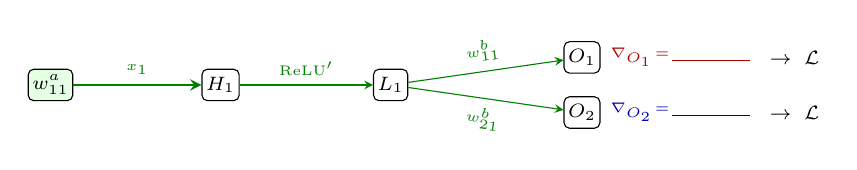
\begin{tikzpicture}[x=1.35cm, y=0.5cm,
  nd/.style={draw, rounded corners=2pt, minimum height=4mm,
             inner sep=1.5pt, font=\scriptsize},
  >=stealth]
\node[nd, fill=green!10] (w) at (0,0) {$w^a_{11}$};
\node[nd] (H) at (1.6,0) {$H_1$};
\node[nd] (L1) at (3.2,0) {$L_1$};
\node[nd] (O1) at (5,0.7) {$O_1$};
\node[nd] (O2) at (5,-0.7) {$O_2$};
\node[font=\scriptsize] at (7, 0.7) {$\rightarrow\;\mathcal{L}$};
\node[font=\scriptsize] at (7,-0.7) {$\rightarrow\;\mathcal{L}$};
\draw[->, green!50!black, thick] (w)--node[above,font=\tiny]{$x_1$}(H);
\draw[->, green!50!black] (H)--node[above,font=\tiny]{ReLU$'$}(L1);
\draw[->, green!50!black] (L1)--node[above,sloped,font=\tiny]{$w^b_{11}$}(O1);
\draw[->, green!50!black] (L1)--node[below,sloped,font=\tiny]{$w^b_{21}$}(O2);
\node[right, font=\tiny, red!70!black] at (O1.east) {$\nabla_{O_1}\!=\!\blk{1cm}$};
\node[right, font=\tiny, blue!70!black] at (O2.east) {$\nabla_{O_2}\!=\!\blk{1cm}$};
%\node[gray, font=\tiny] at (3.2,-1.1) {$\longleftarrow$ gradient flow};
\end{tikzpicture}\vspace{-4pt}
\end{center}


\vspace{-8pt}
\begin{align*}
\frac{\partial\mathcal{L}}{\partial w^a_{11}}
&= \underbrace{\left[\blk{5cm}\right]}_{\nabla_{L_1}}
   \;\cdot\;\;
   \underbrace{\text{ReLU}'(H_1)}_{=\,1}
   \;\cdot\;\;
   \underbrace{x_1}_{=\,0.9} \\[2pt]
&= \bigl[\;\blk{5cm}\;\bigr] \cdot \blk{0.8cm} \cdot \blk{0.8cm}
   =\;\blk{1.5cm}\;
\end{align*}


\vspace{0pt}
\fbox{\parbox{0.96\textwidth}{\small
\textbf{Key Insight --- Initialization Problem:}\;
Based on your computation above, what is the gradient of $w_a$? What does this tell you about weight Initialization? 
\vspace{7pt}
}}



\end{document}
